\documentclass[../main.tex]{subfiles}

\begin{document}


\subsection{Resumen de actividades}

Durante el semestre se trabajó principalmente en realizar correcciones al protocolo de simulaciones y realizar simulaciones de prueba con el protocolo correguido.
Las principales correcciones que se realizaron fueron:
\begin{enumerate}
    \item Correguir la implmentación del potencial de 3 cuerpos en LAMMPS
    \item Cambiar el comando \texttt{write\_data} por el comando \texttt{restart}.
    \item Adaptar el promedio temporal de los commandos \texttt{fix} para los observables de energía y estrés.
    \item Corrección en el cálculo de densidad de empaquetamiento de las simulaciones.
\end{enumerate}
Por otro lado las simulaciones de pruebas fueron realizandose para ir monitoreando que las comabios realizados no alteraran significativamente el comportamiento cualitativo esperado de las relaciones entre deformación y estrés.

Una vez que se implementaron todas las correcciones, se empezaron a realizar simulaciones de exploración de parametros con el objetivo de ir analizando el sistema.
Los parámetros que se variaron fueron el ritmo de deformación y el \texttt{damp}.

\subsection{Resultados principales}

En esta sección se presentan los resultados obtenidos con el protocolo de simulación correguido.
Las simulaciones se realizaron en sistemas de \num{8000} partículas con \num{3}\% de partículas con 4 patches.
Los resultados principales que se presetan son la relación preliminar entre el ritmo de deformación con el estrés en estado estacionario durante una deformación de cizallamiento (figura~\ref{fig:shear-rate-vs-stress}) y la evolución del estrés virial durante una deformación de cizallamiento (figura~\ref{fig:strain-vs-stress}), junto con las correcciones realizadas en el protocolo de simulación con un valor de damp igual a \num{0.1}.

\begin{figure}[h]
    \centering
    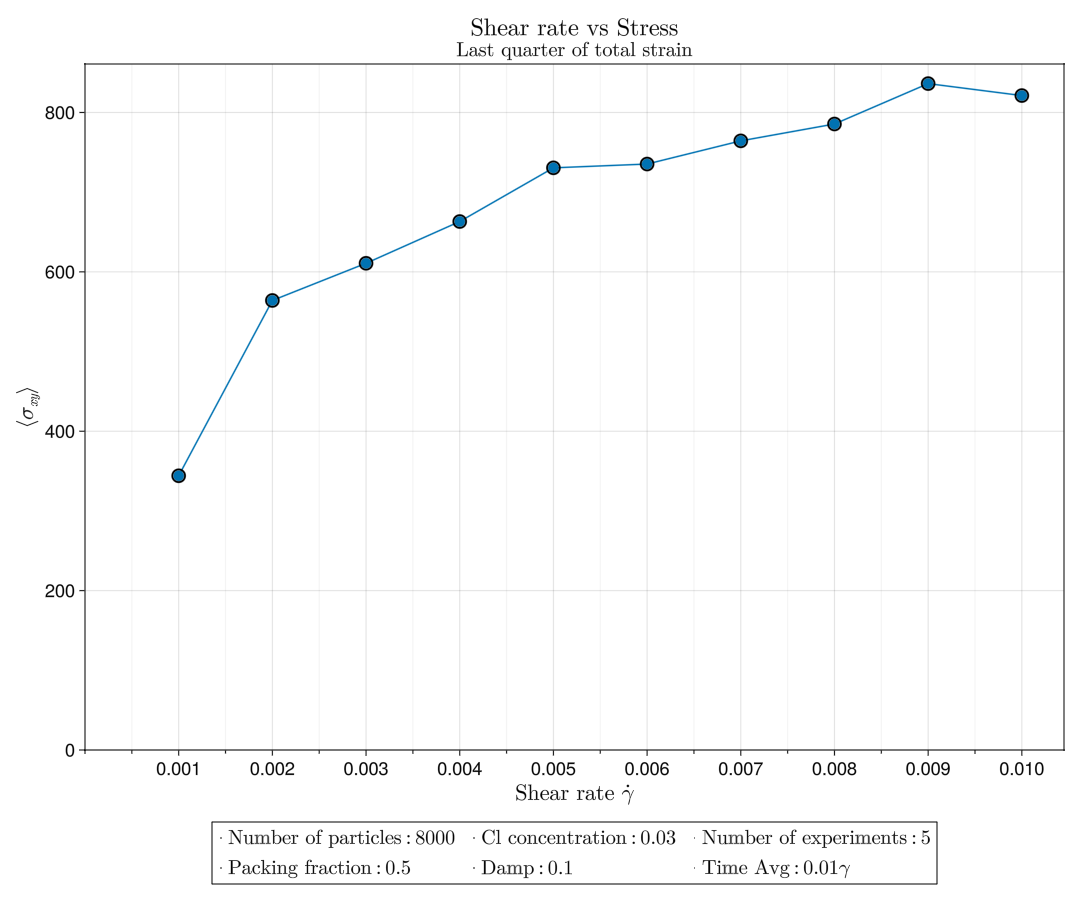
\includegraphics[width=0.9\textwidth]{../Figures/system-2025-05-22-194804-CL-0.03/ShearRate-vs-Stress.png}
    \caption{
        Promedio temporal del estrés en estado estacionario para distintos ritmos de deformación.
    }\label{fig:shear-rate-vs-stress}
\end{figure}

\begin{figure}[h]
    \centering
    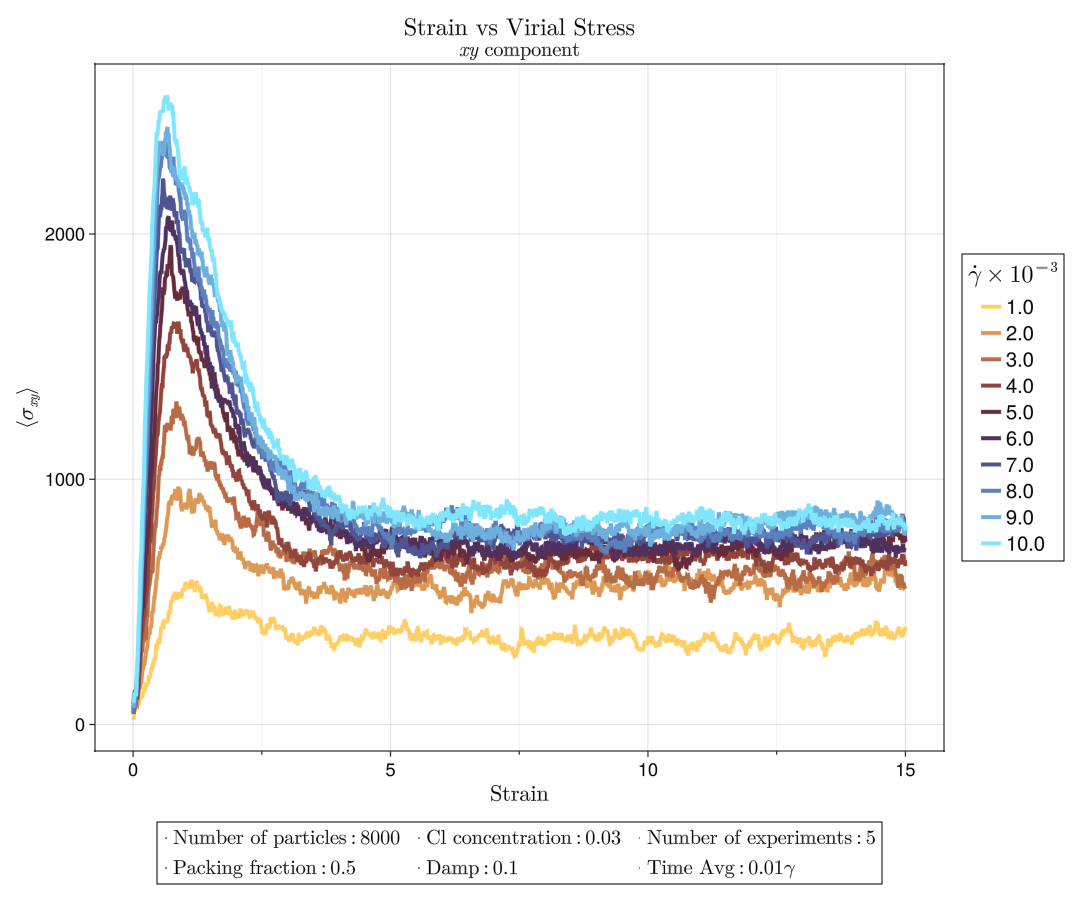
\includegraphics[width=0.9\textwidth]{../Figures/system-2025-05-22-194804-CL-0.03/Strain-vs-StressVirialXY.png}
    \caption{
        Promedio temporal del estrés virial durante una deformación de tipo cizallamiento para distintos ritmos de deformación.
    }\label{fig:strain-vs-stress}
\end{figure}



\subsection{Resultados generales}


\end{document}
